\documentclass[11pt]{article}
\usepackage[a4paper,margin=1in]{geometry}
\usepackage{amsmath,amssymb,amsthm,mathtools}
\usepackage{booktabs}
\usepackage{enumitem}
\usepackage{float}
\usepackage{graphicx}
\usepackage{hyperref}
\usepackage[nameinlink,capitalise]{cleveref}
\usepackage[numbers,sort&compress]{natbib}

\newtheorem{theorem}{Theorem}[section]
\newtheorem{proposition}[theorem]{Proposition}
\newtheorem{corollary}[theorem]{Corollary}
\newtheorem{lemma}[theorem]{Lemma}
\newtheorem{condition}[theorem]{Condition}
\theoremstyle{remark}
\newtheorem{remark}[theorem]{Remark}

\newcommand{\norm}[1]{\left\lVert#1\right\rVert}
\newcommand{\HS}{\mathfrak S_2}
\newcommand{\Id}{I}
\newcommand{\cE}{\mathcal E}
\newcommand{\tr}{\operatorname{tr}}
\newcommand{\spr}{\operatorname{spr}}

\title{Mixed Haar-Channel Riesz Overlap Budgets\\
\large Cross-Stein Identities and a Radial-Block Obstruction}
\author{Liang Wang}
\date{July 2026}

\begin{document}
\maketitle

\begin{abstract}
The remaining analytic premise in the intrinsic small-noise identification
program is a uniform budget for two directional Hilbert--Schmidt Hardy
energies.  The preceding layer showed that a global strong-space mixing rate
spends too much of the available exponent budget, and proposed retaining the
mixed source--resonance--observation overlap of the adjacent Haar channels.

This paper makes that proposal exact at finite dimension.  For a stable
operator and an arbitrary finite Riesz partition, we prove a cross-Stein
identity: the complete Hardy energy is the quadratic form of a positive
semidefinite Gram matrix whose entries are block cross-Gramians.  No
diagonalizability, individual eigenvector normalization, or normality is
required.  A normalized block coherence constant then gives the sufficient
bound
\[
 \cE(r)^2\le \kappa\sum_j K_{jj},
 \qquad
 \kappa=\lambda_{\max}\!\left[
 \frac{K_{jk}}{\sqrt{K_{jj}K_{kk}}}\right].
\]
For simple modes this reduces to the exact Hardy Cauchy kernel
\(\tr(Z_jZ_k^*)/(1-\mu_j\overline{\mu_k}/r^2)\).

We then perform a deterministic all-column binary64 audit on the folded
Gaussian matrices inherited from RH-51.  Fixed radial Riesz blocks preserve
the exact total energies, but their individual block energies and projector
norms become rapidly oblique as the noise decreases.  At the smallest stored
scale the largest radial projector norm is about \(2.7\times10^3\), while the
aggregate left and right energies are only \(1.4681\) and \(1.7603\).  Thus
the cross-Stein theorem identifies the correct signed aggregate object, but a
fixed radial blockwise absolute budget is not a closure of Stage A1.  The
five-scale fits are diagnostics, not asymptotic claims.  A 256-bit Arb audit
certifies the scalar two-block identities only.  Stage A1, intrinsic
identification, any Hilbert--Polya operator, and any arithmetic conclusion
remain open.
\end{abstract}

\noindent\textbf{Keywords:} Hardy energy; Riesz projection; cross-Gramian;
Stein equation; Haar channel; nonnormal operator; small noise.

\medskip
\noindent\textbf{MSC 2020:} 47A10; 47B65; 37D25; 37M25; 65R20.

\section{Introduction}

The fixed-noise intrinsic determinant and its dyadic continuum limit are
rigorous within the transfer-operator model.  The active question is whether
the finite matrix's own Perron/parity-deflated bulk can be identified
uniformly as the Gaussian width tends to zero.  RH-48 reduced this question to
directional reduced resolvents, RH-49 moved the two relevant actions into the
Hilbert--Schmidt class, and RH-50 converted the contour problem into two
time-domain Hardy energies \citep{WangIntrinsic2026,WangDirectional2026,
WangHardy2026}.  RH-51 through RH-56 supplied growing-horizon Stein tails,
peripheral residue transfer, cutoff stability, and a quantitative obstruction
to the global strong-space route \citep{WangStructuredStein2026,
WangFactorTransfer2026,WangHardyTail2026,WangFactorAware2026,
WangRieszCutoff2026,WangHardyBarrier2026}.

Let $T=G_{2n,\sigma}$ and use the adjacent orthogonal Haar decomposition
$V_{2n}=V_n\oplus W_n$.  With $U$ the coarse embedding and $B,C$ the two
off-diagonal Haar couplings, RH-50 studies
\begin{align}
 \cE_B(r)^2
 &=\sum_{m\ge0}r^{-2m}
 \frac{\norm{U^*N_f^mQ_fUB}_{\HS}^2}{\norm B_{\HS}^2},
 \label{eq:left-energy}\\
 \cE_C(r)^2
 &=\sum_{m\ge0}r^{-2m}
 \frac{\norm{CN_c^mQ_c}_{\HS}^2}{\norm C_{\HS}^2}.
 \label{eq:right-energy}
\end{align}
Here $N_f,N_c$ are the intrinsic Perron/parity-deflated fine and coarse
operators and $Q_f,Q_c$ remove the two peripheral ranges.  RH-54 requires a
combined power no larger than $1/4$:
\begin{equation}
 \cE_B(r)=O(\sigma^{-\alpha_B}),\qquad
 \cE_C(r)=O(\sigma^{-\alpha_C}),\qquad
 \alpha_B+\alpha_C\le\frac14.
 \label{eq:budget}
\end{equation}

RH-56 showed that a global strong-space estimate can fail this budget even
when finite-dimensional Hardy traces look modest.  Its surviving suggestion
was to retain the overlap between the special Haar source, the resonance
space, and the observation.  A sum of individual modal bounds is still
unsatisfactory near clustered nonnormal modes.  The present paper therefore
asks for the invariant-block object before any individual eigenvector is
chosen.

\subsection*{Contributions and boundary}

\begin{enumerate}[leftmargin=2.2em]
 \item We prove the cross-Stein Riesz-block identity and the associated
       normalized coherence bound for arbitrary finite stable operators.
 \item We give the simple-mode Hardy Cauchy kernel as a corollary and show
       how growing-horizon block certificates provide diagonal block-energy
       upper bounds.
 \item We implement a grouped left/right invariant-subspace audit which
       checks projector, commutator, partition, Stein, and Gram residuals
       without random trace probes.
 \item We locate a concrete route boundary: fixed radial blocks become highly
       oblique, so their absolute or square-summed budgets do not close the
       small-noise problem even though the signed aggregate Gram quadratic
       form remains modest on the stored levels.
\end{enumerate}

No theorem in this paper establishes a uniform small-noise Hardy bound for
the physical family.  In particular, the numerical projector construction is
not an interval contour proof, and the fitted five-level exponents are not
asymptotic exponents.

\section{Directional Hardy triples}
\label{sec:triples}

For either side of \eqref{eq:left-energy}--\eqref{eq:right-energy}, write the
normalized triple in the common form
\begin{equation}
 \cE(r)^2=\sum_{m\ge0}r^{-2m}\norm{YN^mX}_{\HS}^2,
 \qquad \spr(N)<r,
 \label{eq:common-energy}
\end{equation}
where $(X,Y)=(Q_fUB/\norm B_{\HS},U^*)$ for the left triple and
$(X,Y)=(C^*/\norm C_{\HS},Q_c^*)$ after taking the adjoint for the right
triple.  Put $A=r^{-1}N$.  Then
\begin{equation}
 \cE(r)^2=\sum_{m\ge0}\norm{YA^mX}_{\HS}^2.
 \label{eq:scaled-energy}
\end{equation}
The ordinary controllability Gramian is
\begin{equation}
 G=\sum_{m\ge0}A^mXX^*(A^*)^m,
 \qquad G-AGA^*=XX^*.
 \label{eq:gramian}
\end{equation}
RH-51 used this positive Stein equation for deterministic all-column
calculations.  The issue in the present layer is how to retain the
decomposition of $G$ induced by the bulk resonance space without replacing it
by a global operator norm.

\section{Cross-Stein Riesz identity}
\label{sec:identity}

Let $P_1,\ldots,P_J$ be a Riesz partition of $A$: the projections are
pairwise disjoint, commute with $A$, and sum to the identity on the state
space.  They may be oblique.  Define
\begin{equation}
 X_j=P_jX,\qquad F_j=(YA^mX_j)_{m\ge0}\in\ell^2(\mathbb N_0;\HS).
 \label{eq:block-response}
\end{equation}
The block cross-Gramians are
\begin{equation}
 G_{jk}=\sum_{m\ge0}A^mP_jXX^*P_k^*(A^*)^m.
 \label{eq:cross-gramian}
\end{equation}

\begin{theorem}[Cross-Stein Riesz identity]
\label{thm:cross-stein}
Let $A$ be a finite matrix with $\spr(A)<1$, let $X$ be a finite
Hilbert--Schmidt source, and let $Y$ be a bounded observation.  For any
Riesz partition $\{P_j\}_{j=1}^J$ the series in \eqref{eq:cross-gramian}
converge and satisfy
\begin{equation}
 G_{jk}-AG_{jk}A^*=P_jXX^*P_k^*.
 \label{eq:cross-stein}
\end{equation}
If
\begin{equation}
 K_{jk}:=\tr(YG_{jk}Y^*)
       =\sum_{m\ge0}\tr\!\left(
          YA^mP_jXX^*P_k^*(A^*)^mY^*
        \right),
 \label{eq:block-gram}
\end{equation}
then $K=(K_{jk})$ is positive semidefinite and
\begin{equation}
 \boxed{\cE(r)^2=\sum_{j,k=1}^J K_{jk}.}
 \label{eq:exact-quadratic}
\end{equation}
If $\tr K>0$, define the signed fusion ratio
\begin{equation}
 \eta(K):=\frac{\mathbf 1^*K\mathbf 1}{\tr K}.
 \label{eq:fusion-ratio}
\end{equation}
In particular, if $e_j=K_{jj}^{1/2}$, $D=\operatorname{diag}(e_j)$ on the
nonzero diagonal indices, and $C=D^{-1}KD^{-1}$, then
\begin{equation}
 \boxed{
 \cE(r)^2=\eta(K)\sum_{j=1}^J e_j^2
 \le \lambda_{\max}(C)\sum_{j=1}^J e_j^2.}
 \label{eq:coherence-bound}
\end{equation}
The coarser Gershgorin version is
\begin{equation}
 \lambda_{\max}(C)\le\max_j\sum_k|C_{jk}|.
 \label{eq:gershgorin}
\end{equation}
No diagonalizability or normality assumption is used.
\end{theorem}

\begin{proof}
Since $\spr(A)<1$, the series in \eqref{eq:cross-gramian} converge in finite
dimension.  Separating the first term and shifting the index gives
\eqref{eq:cross-stein}.  The commutation relation $AP_j=P_jA$ gives
\(G_{jk}=P_jGP_k^*\), where $G$ is \eqref{eq:gramian}.  For each $m$ set
$R_{j,m}=YA^mP_jX$.  With the trace inner product linear in its first
argument,
\[
 K_{jk}=\sum_{m\ge0}\tr(R_{j,m}R_{k,m}^*).
\]
Thus $K$ is the Gram matrix of the vectors $F_j$ in
$\ell^2(\mathbb N_0;\HS)$, and summing the responses gives
\eqref{eq:exact-quadratic}.  If $e_j>0$, write $K=DCD$.  The vector of all
ones gives
\[
 \sum_{j,k}K_{jk}=e^*Ce\le\lambda_{\max}(C)e^*e,
\]
Dividing the left side by $\tr K=e^*e$ gives \eqref{eq:fusion-ratio} and
$0\le\eta(K)\le\lambda_{\max}(C)$.  This proves
\eqref{eq:coherence-bound}; Gershgorin gives
\eqref{eq:gershgorin}.  Zero diagonal blocks have zero response and are
removed before forming $D^{-1}$.
\end{proof}

\begin{corollary}[Simple-mode Cauchy kernel]
\label{cor:cauchy}
Suppose $N$ is diagonalizable with simple eigenvalues $\mu_j$, and write
$Z_j=YP_jX$.  Then
\begin{equation}
 \boxed{K_{jk}=\frac{\tr(Z_jZ_k^*)}
 {1-\mu_j\overline{\mu_k}/r^2}.}
 \label{eq:cauchy-kernel}
\end{equation}
For a rank-one projector $P_j=v_j\otimes w_j$ normalized by
$\langle w_j,v_j\rangle=1$,
\begin{equation}
 \norm{Z_j}_{\HS}=\norm{Yv_j}_2\,\norm{X^*w_j}_2.
 \label{eq:rank-one-overlap}
\end{equation}
\end{corollary}

\begin{proof}
In the scaled variable $A=N/r$, $A^mP_j=(\mu_j/r)^mP_j$.
Substitution into \eqref{eq:block-gram} gives the geometric series and
\eqref{eq:cauchy-kernel}.  The rank-one formula follows by factoring
$YP_jX$ into a column and a row.
\end{proof}

\begin{remark}[Interpretation]
The RH-56 modal triangle bound replaces the Gram quadratic form by
\(\sum_j e_j\).  The new sufficient quantity is
\(\sqrt{\kappa\sum_j e_j^2}\), where $\kappa=\lambda_{\max}(C)$.
This can be smaller when block responses are nearly orthogonal.  The exact
factor $\eta(K)$ also retains signed cancellation in the particular aggregate
response, whereas the worst-direction coherence $\kappa$ generally does not.
The worst-direction coherence bound can fail to be useful when a proposed
Riesz partition is highly oblique: the individual $e_j$ can be large even
though their aggregate quadratic form is small.  The exact $\eta$ identity
then points to the missing signed estimate rather than supplying one.
\end{remark}

\section{Block tails and the dyadic target}
\label{sec:target}

Let $A_j=AP_j$ and $X_j=P_jX$.  For an integer $M_j\ge1$, put
\begin{equation}
 S_{j,M_j}=\sum_{m=0}^{M_j-1}A_j^mX_jX_j^*(A_j^*)^m,
 \qquad q_j=\norm{A_j^{M_j}}_2.
 \label{eq:block-prefix}
\end{equation}

\begin{proposition}[Block prefix--tail certificate]
\label{prop:block-tail}
If $q_j<1$, then
\begin{equation}
 K_{jj}\le\tr(YS_{j,M_j}Y^*)+
 \frac{\norm{Y}_{\HS}^2\norm{A_j^{M_j}S_{j,M_j}(A_j^*)^{M_j}}_2}
 {1-q_j^2}.
 \label{eq:block-tail}
\end{equation}
Consequently, diagonal estimates $K_{jj}\le b_j(\sigma)^2$ and a coherence
bound $\kappa(\sigma)\le k(\sigma)$ imply
\begin{equation}
 \cE(r)\le\sqrt{k(\sigma)\sum_jb_j(\sigma)^2}.
 \label{eq:finite-block-target}
\end{equation}
\end{proposition}

\begin{proof}
After time $M_j$, the state is $A_j^{M_j}$ applied to a prefix state.  The
tail controllability Gramian is bounded by the geometric Neumann series with
ratio $q_j^2$.  Taking the observed trace gives \eqref{eq:block-tail}; insert
the diagonal bounds into \eqref{eq:coherence-bound} for the last statement.
\end{proof}

The resulting sufficient condition is sharper than the RH-56 absolute modal
sum, but it is still a condition rather than a physical-family theorem.  A
direct signed route may replace $\kappa$ below by a proved upper for the
specific Rayleigh ratio $\eta(K)$; that estimate must control the cross terms,
not infer cancellation from finite data.

\begin{condition}[Cross-Stein overlap budget]
\label{cond:cross-budget}
At every required small-noise level, choose invariant blocks for the left and
right triples so that
\begin{equation}
 \kappa_B(\sigma)\sum_jK_{B,jj}(\sigma)=O(\sigma^{-2\alpha_B}),
 \qquad
 \kappa_C(\sigma)\sum_jK_{C,jj}(\sigma)=O(\sigma^{-2\alpha_C}),
 \label{eq:cross-budget}
\end{equation}
with $\alpha_B+\alpha_C\le1/4$.  The constants and block construction must
be uniform over the dyadic schedule.
\end{condition}

\begin{corollary}[Implication for Stage A1]
Condition \cref{cond:cross-budget}, together with the RH-50 contour Hardy
upper and the RH-52--RH-55 peripheral, factor, and cutoff interfaces, closes
the Hardy portion of intrinsic identification at the stated exponents.  A
bounded or polylogarithmic $\kappa$ with square-summed block energies is
sufficient; it is not proved here for the physical family.
\end{corollary}

\begin{proof}
Apply \cref{thm:cross-stein} to the normalized left and right triples.  The
two square roots in \eqref{eq:cross-budget} give the two Hardy powers, whose
sum is at most $1/4$.  The remaining interfaces are precisely those already
established in the cited layers.
\end{proof}

\section{Binary64 grouped-block audit}
\label{sec:numerics}

We use the folded midpoint Gaussian matrices from RH-51 and RH-53.  The
fine dimensions satisfy $N\sigma=5.12$ at
\[
 (\sigma,N)=(0.16,32),(0.08,64),(0.04,128),(0.02,256),(0.01,512).
\]
The Perron and negative parity branches are removed by the biorthogonal
rank-two subtraction used in those layers.  The left operator is $N_f/0.85$
with source $Q_fUB/\norm B_{\HS}$ and observation $U^*$.  The right operator
is $N_c^*/0.85$ with source $C^*/\norm C_{\HS}$ and observation $Q_c^*$.

For each triple, the bulk spectrum is grouped by physical modulus using the
fixed cuts $0.15,0.35,0.55$.  The groups are called central, inner cloud,
middle cloud, and edge cloud; empty groups are omitted.  A noncentral
projector is formed from paired left and right eigenspaces, and the central
projector is the complement of their sum.  This is a grouped invariant-
subspace construction, not a sum of individual eigenvector condition
numbers.

The full controllability Gramian is solved densely in binary64 and every
source column is included.  We form the block Gram matrix from
\[
 K_{jk}=\tr(YP_jGP_k^*Y^*).
\]
The audit records Stein, partition, commutator, and Gram residuals.

\begin{table}[H]
\centering
\scriptsize
\begin{tabular}{@{}r|rr|rr|rr|rr@{}}
\toprule
 & \multicolumn{2}{c|}{exact $\cE$} & \multicolumn{2}{c|}{square sum}
 & \multicolumn{2}{c|}{coherence upper} & \multicolumn{2}{c}{max $\norm P_j$}\\
 $\sigma$ & left & right & left & right & left & right & left & right\\
\midrule
0.16 & 0.9040 & 1.0026 & 1.4992 & 1.8343 & 1.9188 & 2.3977 & 4.21 & 4.03\\
0.08 & 1.1626 & 1.2653 & 2.2621 & 4.2979 & 2.9871 & 5.8984 & 13.30 & 13.55\\
0.04 & 1.3338 & 1.4845 & 4.3864 & 8.9683 & 6.1122 & 12.7305 & 51.45 & 48.42\\
0.02 & 1.4096 & 1.6340 & 28.9725 & 127.4598 & 40.9396 & 180.2447 & 845.82 & 835.67\\
0.01 & 1.4681 & 1.7603 & 57.6743 & 474.0177 & 81.6785 & 672.4059 & 2705.75 & 2531.73\\
\bottomrule
\end{tabular}
\caption{Grouped radial Riesz audit at $r=0.85$.  The exact column is the
direct all-column Lyapunov energy.  The square-sum column is
$\sqrt{\sum_jK_{jj}}$, and the coherence column is
$\sqrt{\lambda_{\max}(C)\sum_jK_{jj}}$.  The last columns show the largest
oblique projector norm.  All entries are binary64 diagnostics.}
\label{tab:main-audit}
\end{table}

The block identity is numerically stable on these levels.  The maximum
relative reconstruction defect is $1.83\times10^{-12}$ and the maximum
partition defect is $6.2\times10^{-14}$.  The large upper bounds in
\cref{tab:main-audit} are therefore not caused by omitted source columns;
they are caused by the oblique invariant-block decomposition.

The fitted log--log slopes of the exact left and right energies are $0.168$
and $0.199$ over these five levels.  The corresponding slopes for the
coherence upper are approximately $1.46$ and $2.12$.  These are descriptive
finite-range fits only.  The exact-energy fit is not an asymptotic theorem,
and the rapidly growing block upper is not a proof that the physical Hardy
energies diverge.

\begin{figure}[H]
\centering
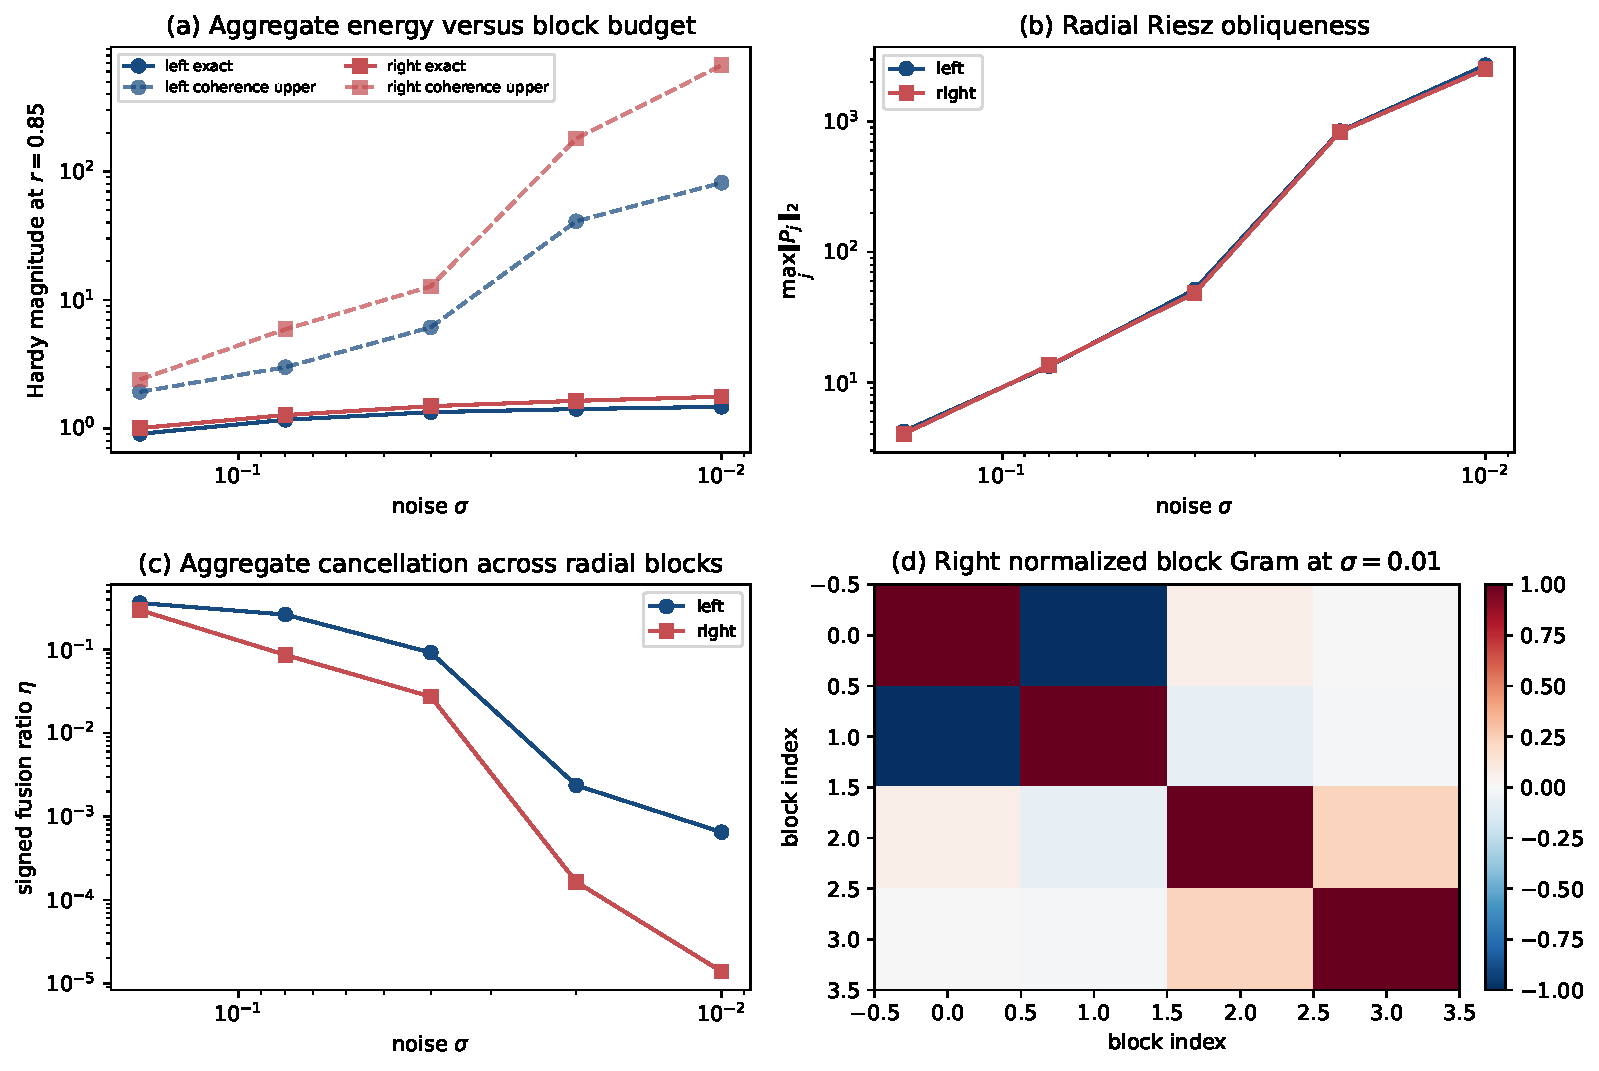
\includegraphics[width=\textwidth]{figures/mixed_haar_channel_overlap.pdf}
\caption{Grouped-block audit.  (a) The signed aggregate Lyapunov energies
remain below the coherence-weighted radial-block upper.  (b) Radial Riesz
projectors become strongly oblique.  (c) The signed fusion ratio decreases as
large radial block responses cancel in the aggregate.  This is a diagnostic,
not a uniform cancellation theorem.  (d) Right-channel normalized block Gram
at $\sigma=0.01$.}
\label{fig:audit}
\end{figure}

All production eigenspaces, Lyapunov solutions, and singular norms are
binary64 and are not interval enclosures.  A separate 256-bit Arb calculation
evaluates a two-mode real model with
\[
 \mu_1=0.72,\qquad \mu_2=-0.61,\qquad Z_1=0.37,\qquad Z_2=-0.29,
\]
and certifies positivity of its cross-Gram matrix, the geometric-series
Cauchy entries, and the coherence and triangle inequalities.  It does not
enclose a production Riesz projector.

\section{Route consequence}
\label{sec:consequence}

\begin{description}[leftmargin=4.7cm,style=nextline]
 \item[Global strong-space black box]
 Quantitatively obstructed by RH-56; this paper does not reopen that route.
 \item[Individual modal absolute overlaps]
 Too sensitive to clustered nonnormal eigenvectors and not needed for the
 exact finite-dimensional identity.
 \item[Fixed radial Riesz blocks]
 Not a uniform closure route in the present audit.  Their projector norms and
 diagonal block energies grow rapidly, even though the signed aggregate is
 moderate.
 \item[Cross-Stein aggregate]
 The invariant target is the quadratic form $\mathbf 1^*K\mathbf 1$, or a
 uniform upper obtained from normalized coherence and diagonal block energies.
 \item[Stage A1]
 Open.  \cref{cond:cross-budget} is a sharper sufficient condition, not a
 theorem for the physical small-noise family.
 \item[Stage A4 intrinsic identification]
 Still conditional on Stage A1.  RH-52--RH-55 close the peripheral, factor,
 and adaptive-cutoff interfaces once the Hardy budget is supplied.
\end{description}

The next meaningful gate is an angular or time-ordered block construction
with uniform separation, a direct signed cross-Stein estimate, or a validated
Schur/Gramian formulation that avoids individual spectral coordinates.  Merely
increasing the precision of the current five-scale eigensolver would not
establish a dyadic theorem.

\section{No arithmetic or Hilbert--Polya conclusion}

Nothing here supplies a von Mangoldt or prime-power trace formula, a zeta-zero
spectral identity, a canonical self-adjoint operator, or a $T\log T$ counting
law.  No Riemann-hypothesis conclusion is drawn.  The independent twin-prime
branch is not used.  This is a transfer-operator Hardy/Riesz route analysis
and a delimited negative diagnostic for one block choice.

\section{Reproducibility}

The directory contains the source algebra, tests, five-scale all-column
results, the Arb scalar certificate, figure, publication hashes, and archive
verification.  The principal commands are:
\begin{verbatim}
PYTHONDONTWRITEBYTECODE=1 /root/math/.venv/bin/pytest -q -p no:cacheprovider
PYTHONDONTWRITEBYTECODE=1 /root/math/.venv/bin/python \
  experiments/run_overlap_pilot.py
PYTHONDONTWRITEBYTECODE=1 /root/math/.venv/bin/python \
  experiments/run_arb_block_audit.py
MPLBACKEND=Agg PYTHONDONTWRITEBYTECODE=1 /root/math/.venv/bin/python \
  experiments/make_figures.py
latexmk -pdf -interaction=nonstopmode -halt-on-error main.tex
\end{verbatim}

The theorem, cross-Stein identities, and scalar Arb formulas are exact in
their stated finite-dimensional scope.  The grouped production eigendata are
binary64 evidence only.  Stage A1, unconditional intrinsic identification,
any self-adjoint Hilbert--Polya realization, and all arithmetic conclusions
remain outside the claims.

\bibliographystyle{plainnat}
\bibliography{references}
\end{document}
